%!TEX root = ./main.tex

%** Results.tex: What were the results achieved including an evaluation

\chapter{Results and Evaluation\label{Results}}

\section{Results}
\subsection{IPv6 and the SWITCH network\label{RES_IPV6}}
\begin{figure}[hb!]
	\centering
	\includegraphics[height=70mm]{images/overview_v4v6}
	\caption{Comparison of the traffic levels of IPv4 and IPv6 in the SWITCH network in terms of connections per 5 minutes}
	\label{fig:ipv6_switch}
\end{figure}
This section is to get an idea of the deployment of IPv6 in the SWITCH network at the end of August 2010. As figure \ref{fig:ipv6_switch} shows that there are around 8M-20M IPv4 connections per 5 min time slot. On the other hand, there are only 50k-100k IPv6 connections per 5 min time slot. So the overall traffic level of IPv4 is a factor 160 - 200 higher than the traffic level of IPv6. This means that there is at least 160 times more IPv4 traffic than IPv6 traffic. Consequently, FACT has some trouble in detecting connectivity issues in IPv6 networks with the same reliability as in IPv4 networks because of this significant lower traffic volume, i.e. most likely due to a significant lower number of IPv6 user.

\subsection{Analysis of a two week traffic trace}
In order to demonstrate how efficient and comfortable FACT works in practice, a few details of a two week traffic trace from the entire SWITCH network are elaborated. This traffic trace has started on 30/08/2010 at midnight and ended around 12 days later on 11/09/2010. Since FACT is analyzing the data split up in 5 minute time slots, there are 3492 reporting files generated.

\subsubsection{Data}
SWITCH is collecting unsampled traffic traces at their boarder router which exports netflow traces to a central instance within the SWITCH network. They are saved so that these traces are available for several years back. The CSG has an exclusive access to this traffic traces in order to a research contract with SWITCH.

\subsubsection{IPv4}
A brief statistic of this two week IPv4 traffic trace:
\begin{itemize}
	\item 2170 time slots are classified as \texttt{UNLIKELY}, this yields that there are no problems reported in 62\% of the time (180 hours within 291 hours).
	\item 912 time slots are classified as \texttt{LIKELY}. In 26\% of the cases there may be a connectivity issue. However, some further investigation is required to definitely denote a connectivity problem within these time slots.
	\item 410 time slots are classified as \texttt{VERY LIKELY}. Hence, in 34 hours (11\%) of the trace a connectivity issue is reported.
\end{itemize}

Figure \ref{fig:ipv4_prefix_failed} is presenting the number of failed prefixes over time. This semi-log plot shows how many external prefixes are classified as unreachable over time. The severity is indicated by colors, red stands for $severity \ge 1$ which means that at least one host is affected by the given number of failed prefixes. According to that, green stands for $severity \ge 2$, blue for $severity \ge 5$ and purple for $severity \ge 10$. It is visible that the red curve is heavily fluctuating, because there is a high impact of some noise like port scans, DDoS backscatter, etc. Consequently, the green curve is showing the number of failed external prefix whose outage affects two or more internal hosts. This is to be considered as more robust to noise. Therefore, if at least 10 internal hosts are affected one is attempted to state that this is certainly a real connectivity problem. Hence, for each purple spot there may be a connectivity issue on a very high probability.
\begin{figure}[hb!]
	\centering
	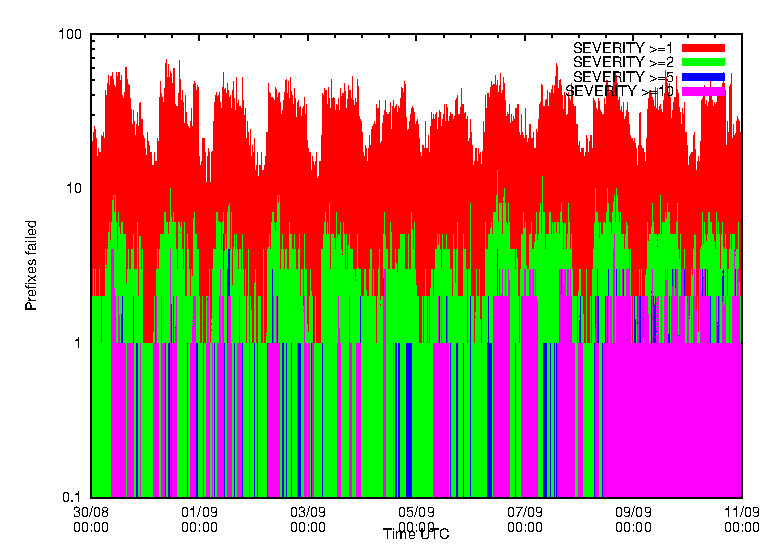
\includegraphics[height=75mm]{images/prefix_failed_ipv4.eps}
	\caption{number of failed IPv4 prefixes within the two week traffic trace}
	\label{fig:ipv4_prefix_failed}
\end{figure}

\subsubsection{IPv6}
Figure \ref{fig:ipv6_prefix_failed} is showing again how many external prefixes are classified as unreachable, but for IPv6 instead of IPv4 as in figure \ref{fig:ipv4_prefix_failed}. Obviously, there are hardly any IPv6 connectivity issues detected in contrast to the IPv4 plot. This may be a result of the low traffic level of IPv6 in the SWITCH network or just because there are no severe connectivity issues within the observed timeframe. The red spots which can be seen on figure \ref{fig:ipv6_prefix_failed} are prefix failures which only affect one internal host and this is - as stated above - not very reliable. Moreover, there are five green spots which indicate a prefix failure which affects 2 or more internal hosts. Further investigation though yields that these spots are caused by the same two hosts within a single /48 network. This may be a real connectivity issue. However, only two internal hosts are affected by this problem which is of course still not as reliable as severity 10.

\begin{figure}[hb!]
	\centering
	\includegraphics[height=80mm]{images/prefix_failed_ipv6.eps}
	\caption{number of failed IPv6 prefixes within the two week traffic trace}
	\label{fig:ipv6_prefix_failed}
\end{figure}

\section{Evaluation}
As the two plots above shows, prefix failures may be extracted quite well with FACT. So further investigation of the problematic time instances is needed. This may be done through the consultation of the report file of these time slots. At 30/08/2010 11.15 CEST for example there are 4 IPv4 prefixes reported as failed with $severity \ge 10$ . The investigation yields that some prefixes of a content distribution network provider have not been reachable during 2 hours and thus, caused that some content of this provider and their customers were partially unavailable. The larger purple blocks around the 08/09/2010 till the 11/09/2010 exhibits again one of these prefixes as broken. This shows that it was not possible to completely resolve that problem within at least 12 days. If FACT were deployed at that moment, this prefix failure, which may be a result of a broken peering or another routing failure, would have been resolved faster.

This analysis of the two week trace shows how easy it is to classify and identify connectivity issues with FACT. However, FACT requires a certain level of traffic to reliably classify connectivity issues. Moreover, there are some methodical details to evaluate:
\begin{itemize}
	\item How precise is the classification of connectivity issues?
	\item How complete is the classification of connectivity issues?
	\item How low is the false positive rate?
\end{itemize}

\subsection{Precision}
The precision is defined as the fraction of the true positives and the sum of the true positives and the false positives. Further investigation of the report files and of the above plot yields that there are hardly any False Positives in this data set which leads to a very low false positive. Therefore, the Precision should be quite high, at least if there is enough traffic to get a high severity.

\subsection{Recall}
The recall is an indicator for the completeness of the connectivity issue tracking. Firstly, the complete set of connectivity issues has to be defined. Either all connectivity issues of the entire Internet are defined as set of connectivity issues or all connectivity issues which concern the network users. In the first case the recall would be very low, because it is very unlikely that the connections of all internal users will track all connectivity issues in the entire Internet. Consequently, there are a lot of false negatives and therefore, the recall is very low. The second case is harder to examine and needs a very detailed examination which will not fit the extent of this thesis. This is due to the uncertainty of how robust and reliable the severity one is. If all connectivity issues of severity one are considered, the false negatives will increase by this amount what decreases the recall in turn.

\subsection{False Positive Rate}
To determine the false positive rate the robustness and significance of the severity has to be estimated again. Since the consideration of severity one will lead to a high number of false positives due to port scans or other blocked traffic, the false positive rate will be higher than in the cases of severity bigger than one. This assumes that the likelihood of independently creating scanning traffic or some blocked traffic towards the same external network by two or more internal hosts is very low. Nevertheless, relying on a severity bigger than one should lead to a quite low false positive rate. However, there is a conflict between the false positive rate and the recall. The overall traffic level impacts again the ability to aggregate prefix failures by internal hosts. The higher the traffic level is, the higher the probability to aggregate a prefix failure to more than one host and the more reliable a classification gets.
